%--------------------------------------------------------------------
%--------------------------------------------------------------------
% Formato para los talleres del curso de Métodos Computacionales
% Universidad de los Andes
%--------------------------------------------------------------------
%--------------------------------------------------------------------

\documentclass[11pt,letterpaper]{exam}
\usepackage[utf8]{inputenc}
\usepackage[spanish]{babel}
\usepackage{graphicx}
\usepackage{tabularx}
\usepackage[absolute]{textpos} % Para poner una imagen en posiciones arbitrarias
\usepackage{multirow}
\usepackage{float}
\usepackage{hyperref}
%\decimalpoint

\begin{document}
\begin{center}
{\Large Métodos Computacionales} \\
\textsc{Tarea 2}\\
01-2019\\
\end{center}

\noindent
\section{Ejercicio 2: Transformada de Fourier}
\begin{center}
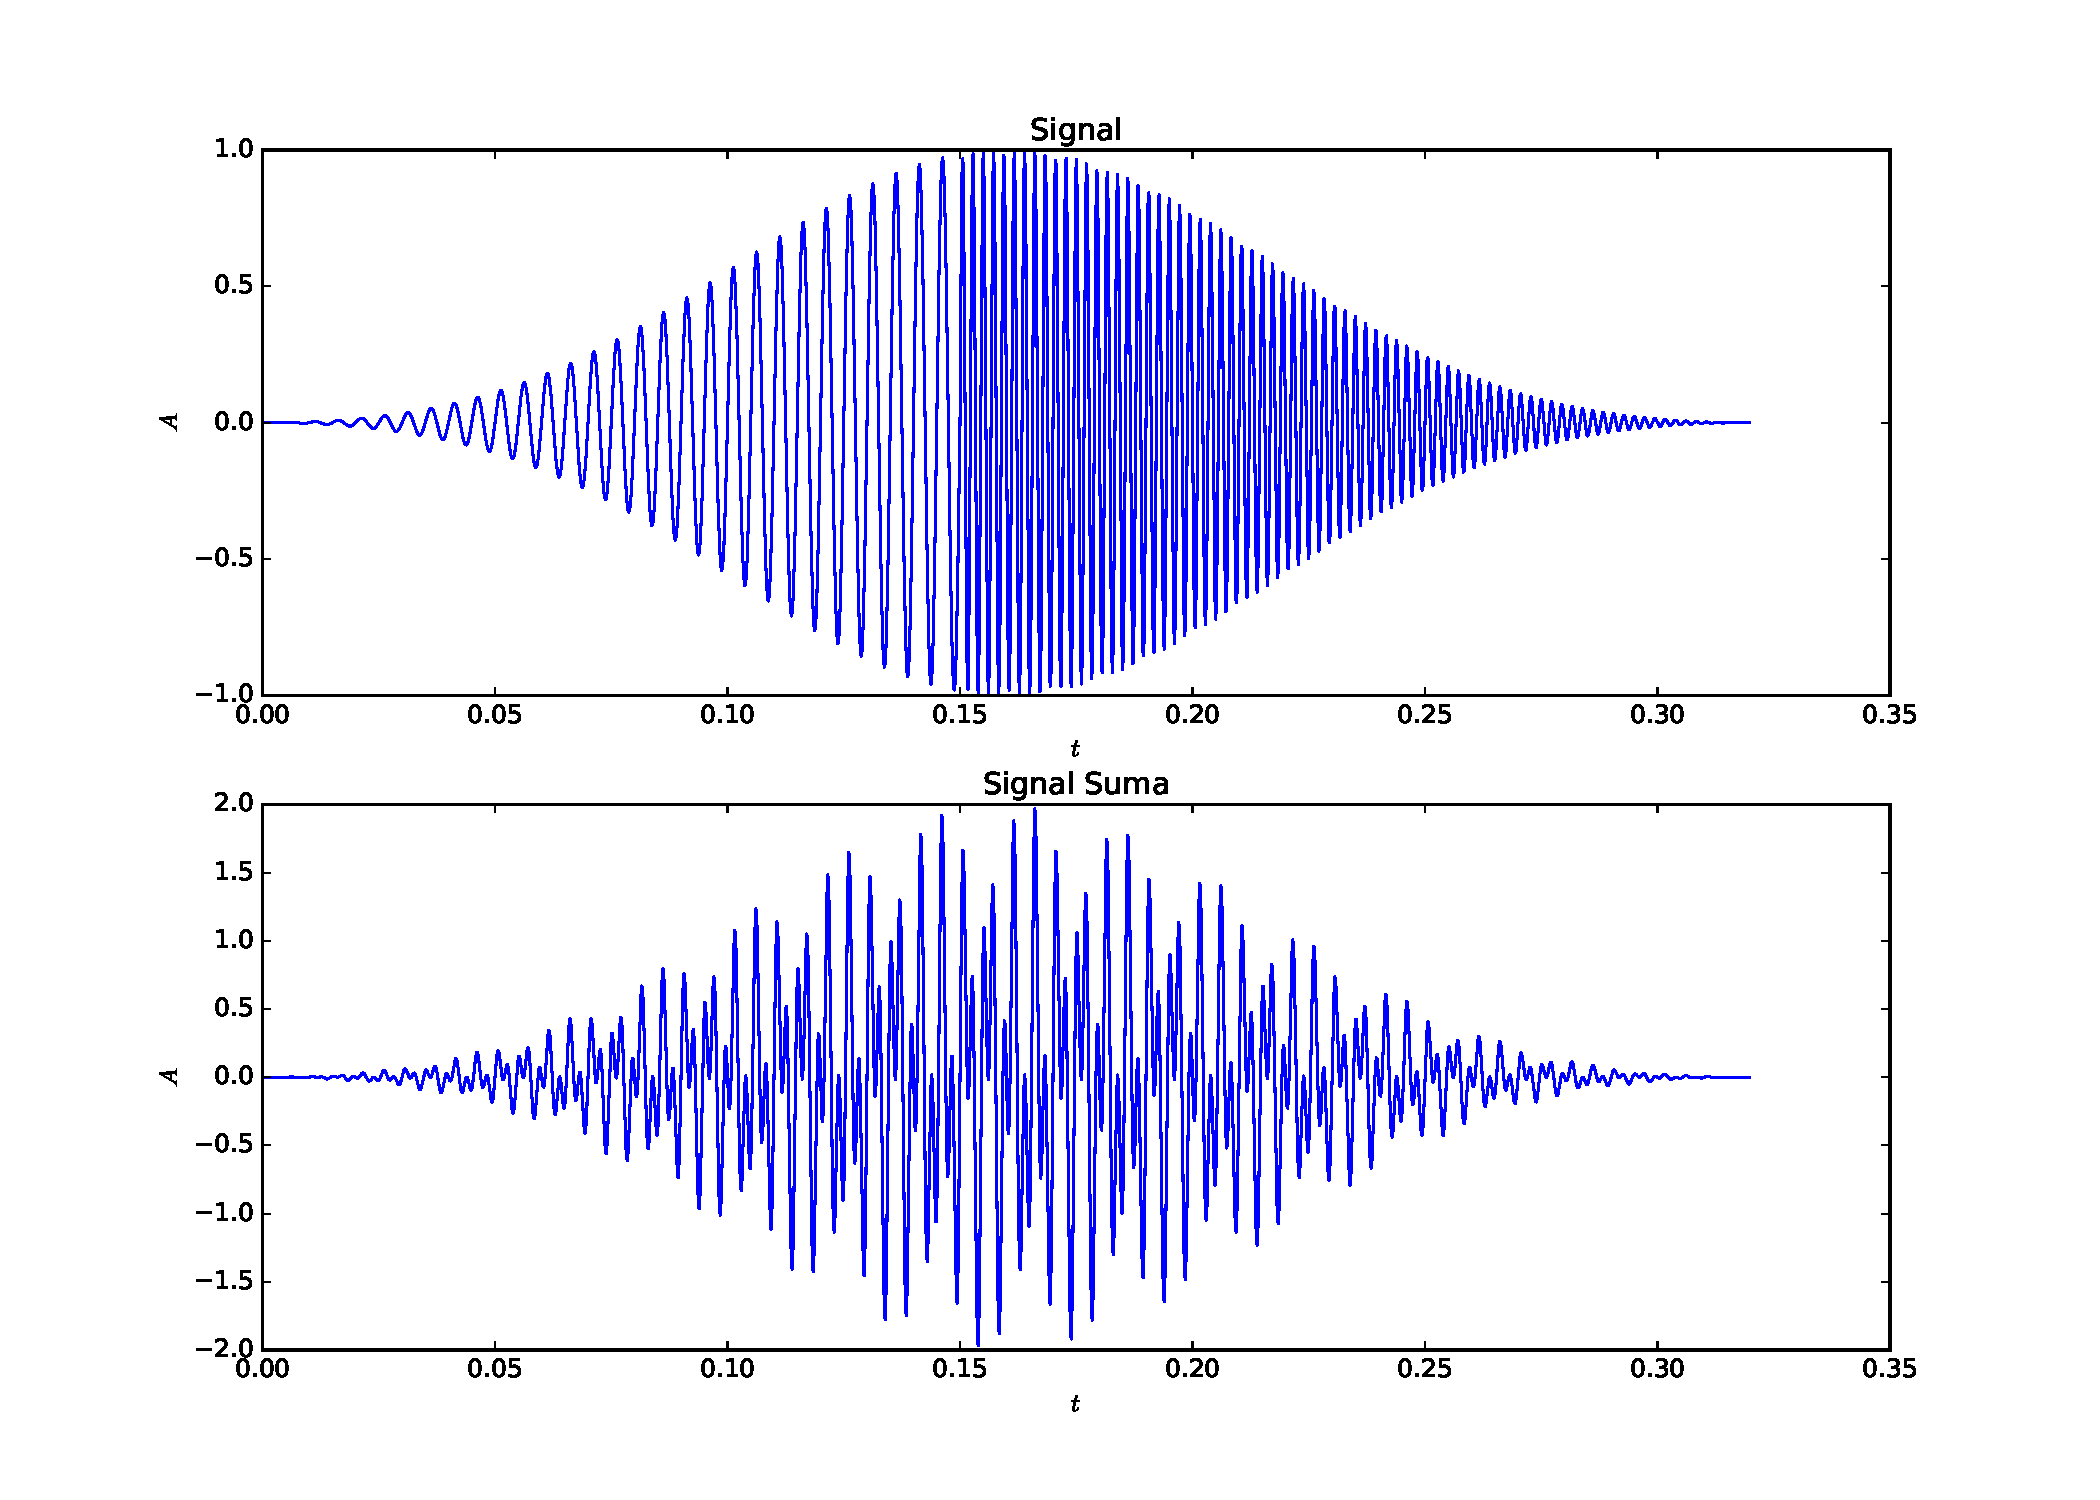
\includegraphics[width=14cm]{2_Signal.pdf} 
\end{center}
{Gráficas de las señales 'Signal' y 'SignalSuma'. Cualitativamente podemos ver que 'Signal' cambia de frecuencia 'principal' en $t=0.15$, mientras que 'SignalSuma' es la suma de dos señales con frecuencias distintas. } 
\begin{center}
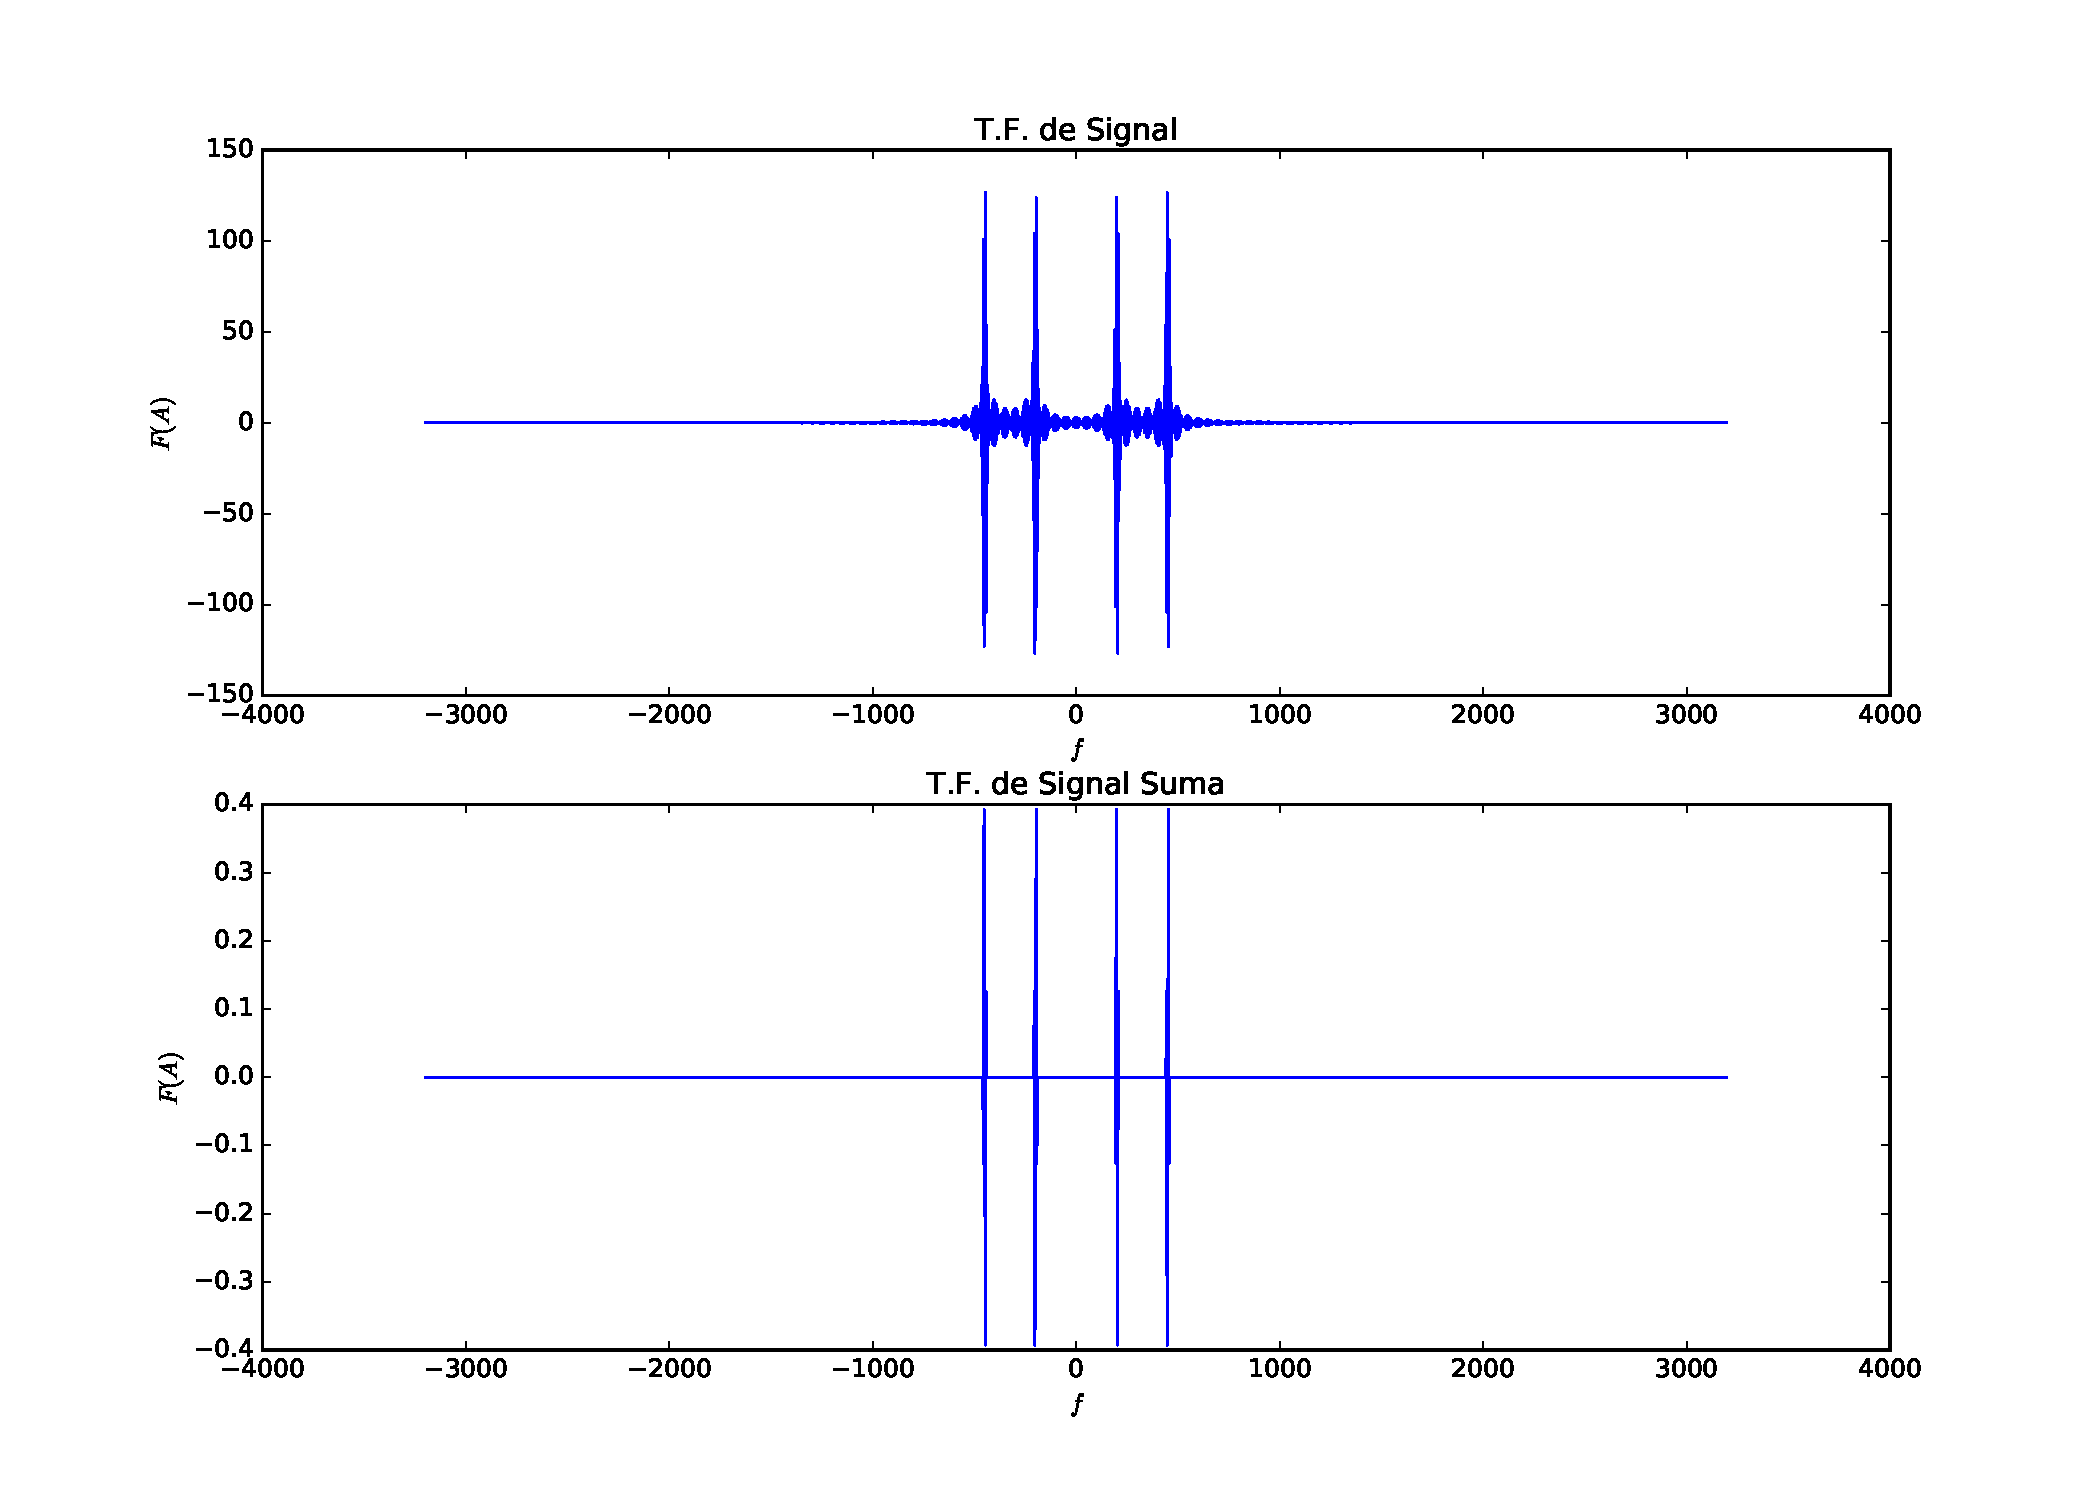
\includegraphics[width=14cm]{2_FourierSignal.pdf} 
\end{center}
{Transformadas de Fourier de 'Signal' y 'SignalSuma'. Aqu\'i es claro que Signal se compone de dos frecuencias principales $\sim \pm 200, \pm 400$, pero hay ciertas frecuencias intermedias que realizan el cambio que hemos mencionado. Por otro lado, SignalSuma sólo se compone de la superposición de dos frecuencias $\sim \pm 200, \pm 400$.}
\begin{center}
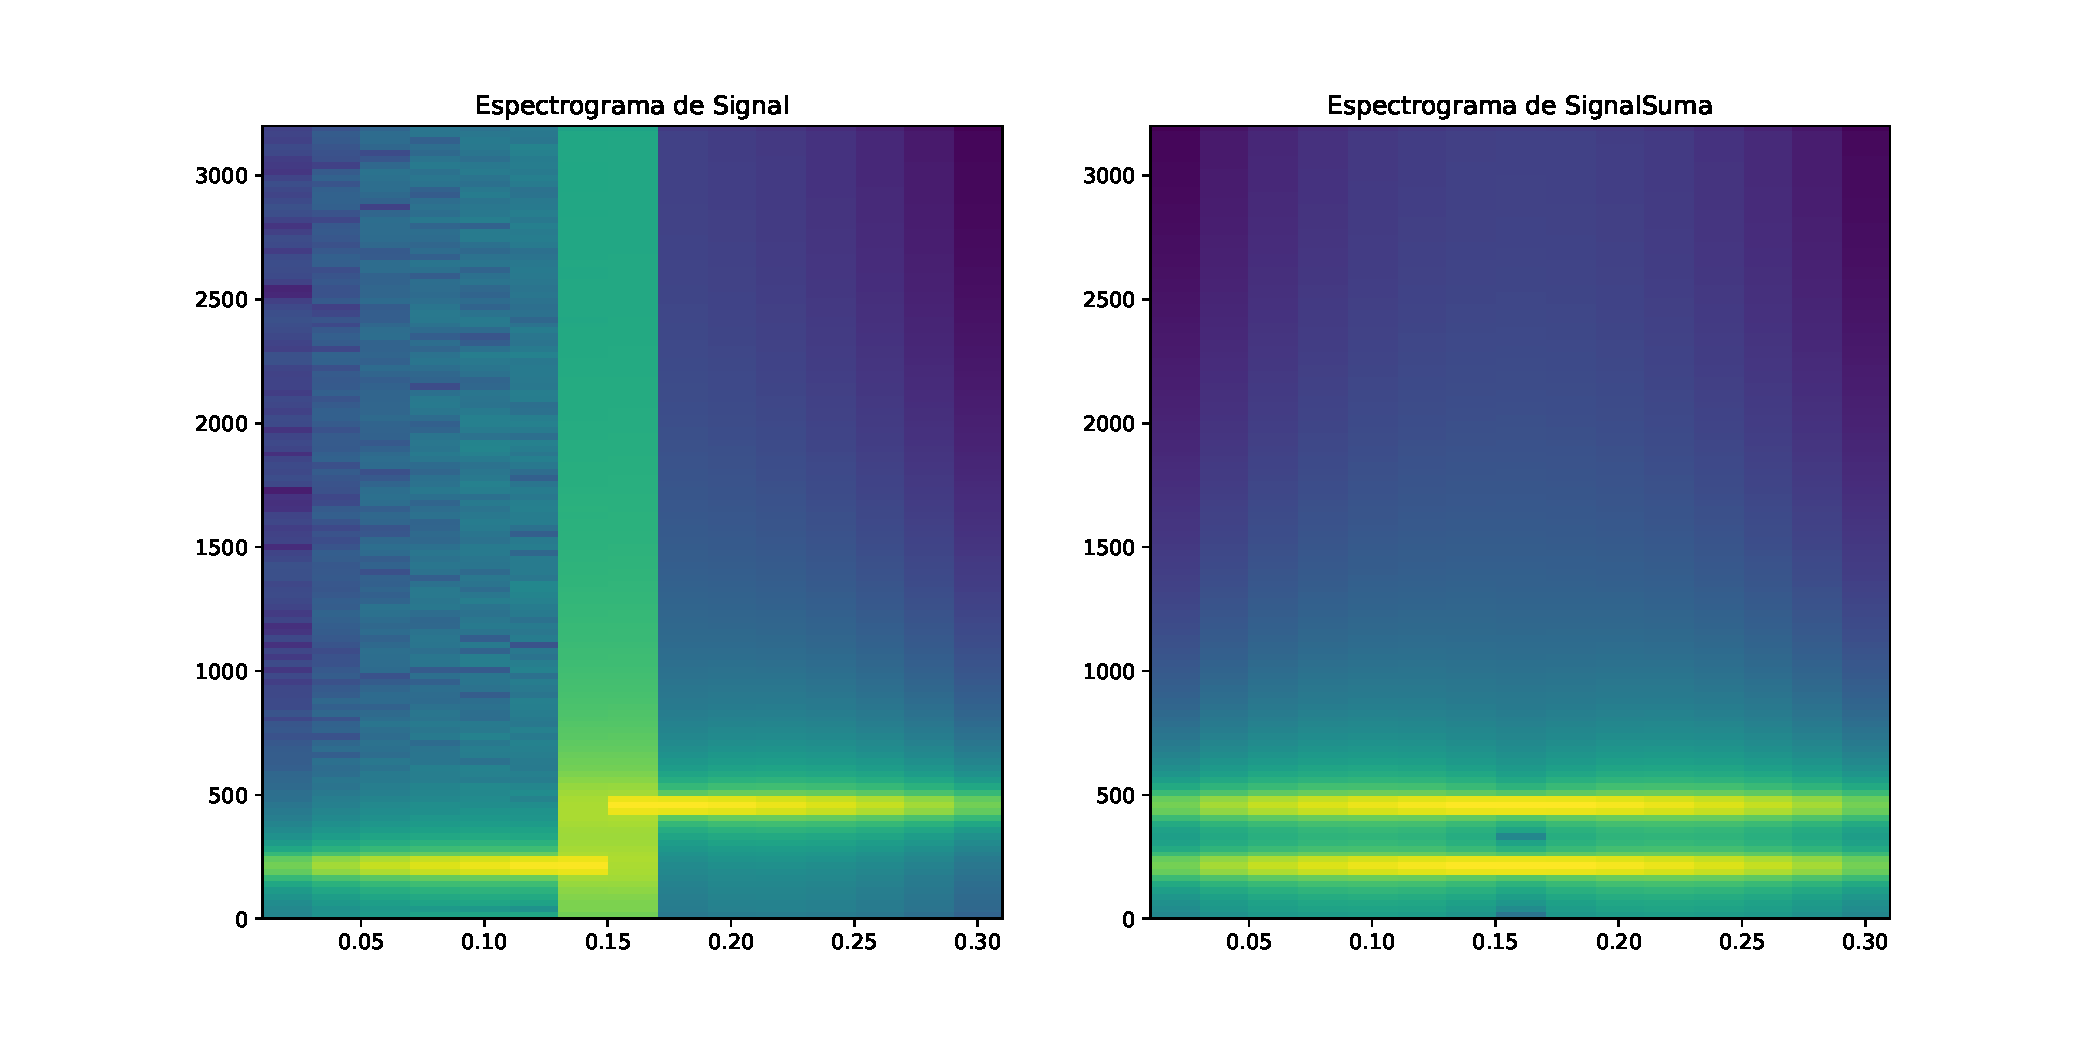
\includegraphics[width=14cm]{2_Espectrogramas.pdf} 
\end{center}
{Espectrogramas de Signal y SignalSuma. El espectrograma mapea la intensidad de cada una de las frecuencias individuales en cada momento $t$. Para Signal se ve la transici\'on de $\sim 200$ a $\sim 400$ alrededor de 0.15, donde tiene una breve superposición de ambas. Por otro lado, para SignalSuma es claro que las dos frecuencias que la componen están superpuestas en todo momento, como esper\'abamos.}
\begin{center}
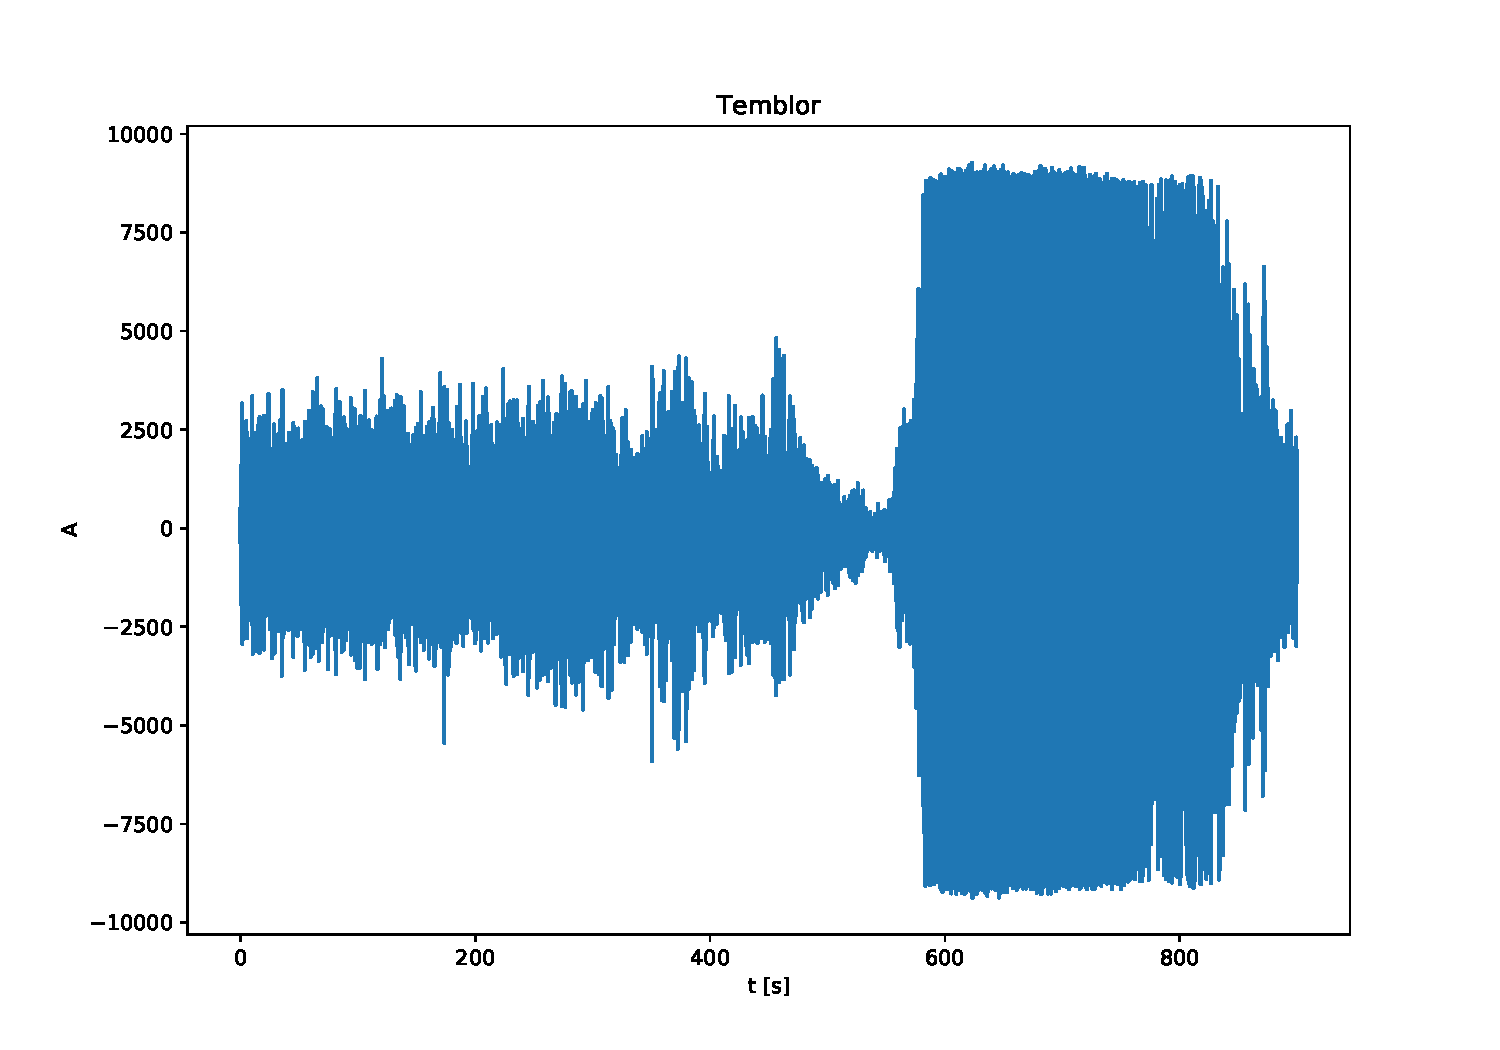
\includegraphics[width=14cm]{2_Temblor.pdf} 
\end{center}
{Gráfica de la señal del temblor. En principio no es muy claro de qué frencuencias se compone.}
\begin{center}
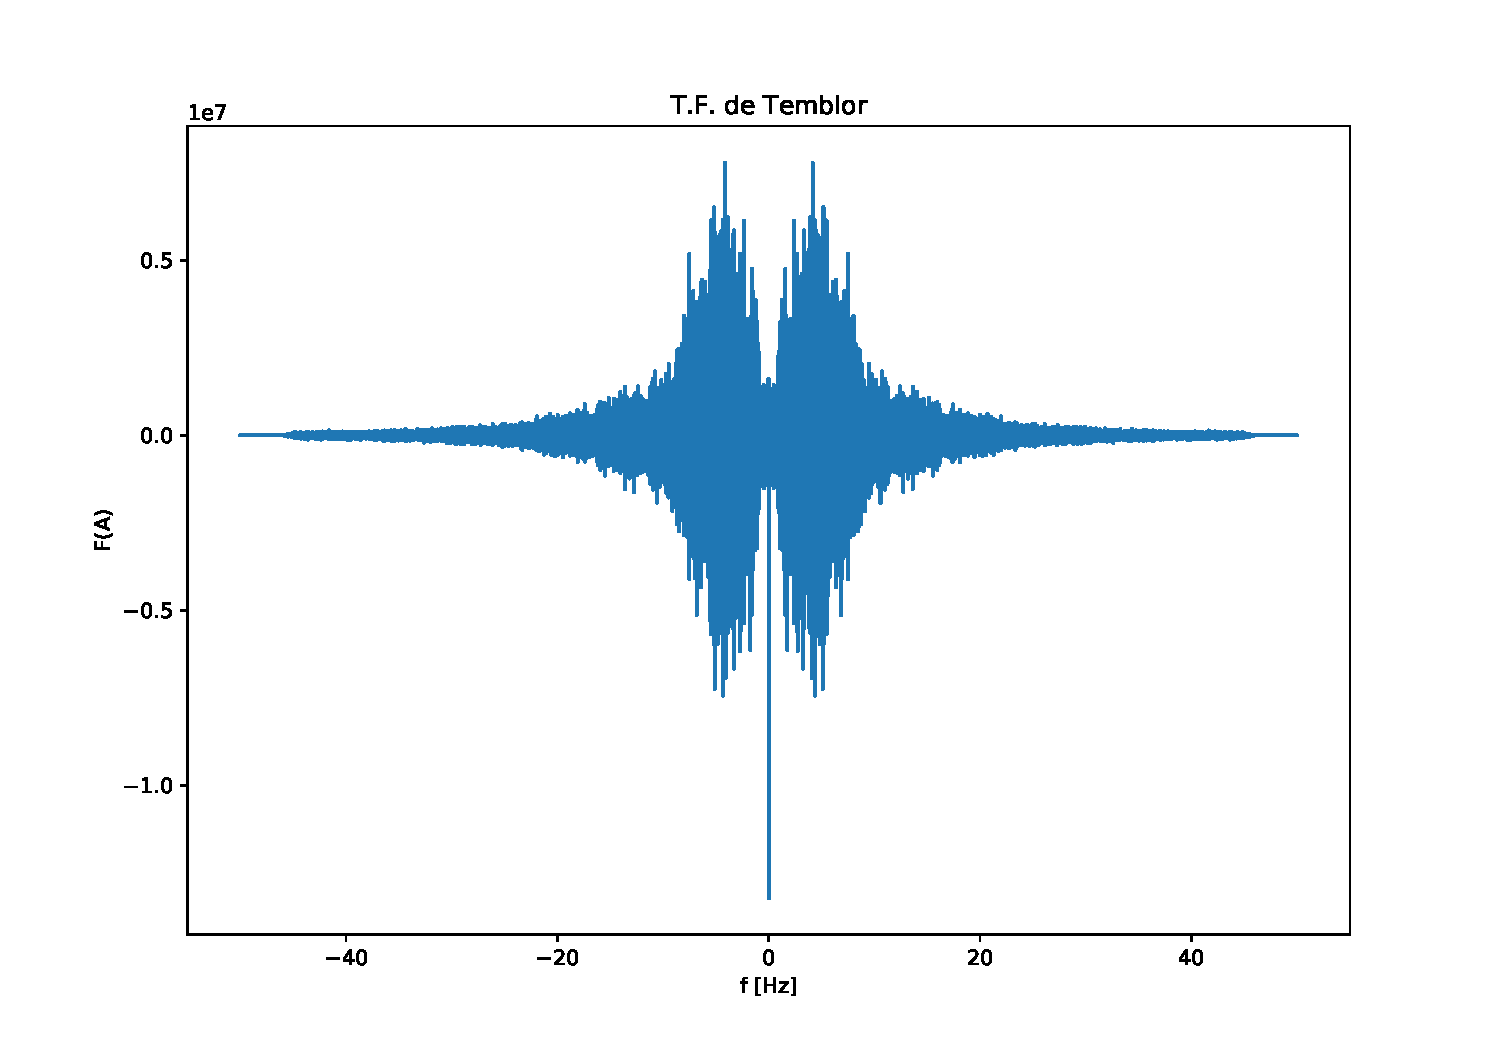
\includegraphics[width=14cm]{2_FourierTemblor.pdf}
\end{center}
{Transformada de Fourier del temblor. Acá se puede ver que hay una concentración de frecuencias alrededor de $\sim\pm 0.0005$. la cual podría considerarse como ' la frecuencia principal' del temblor. Tiene sentido que la frecuencia sea muy pequeña, pues las ondas sísmicas de un temblor deben tener longitudes do onda en el orden de kilómetros, por lo menos.}
\begin{center}
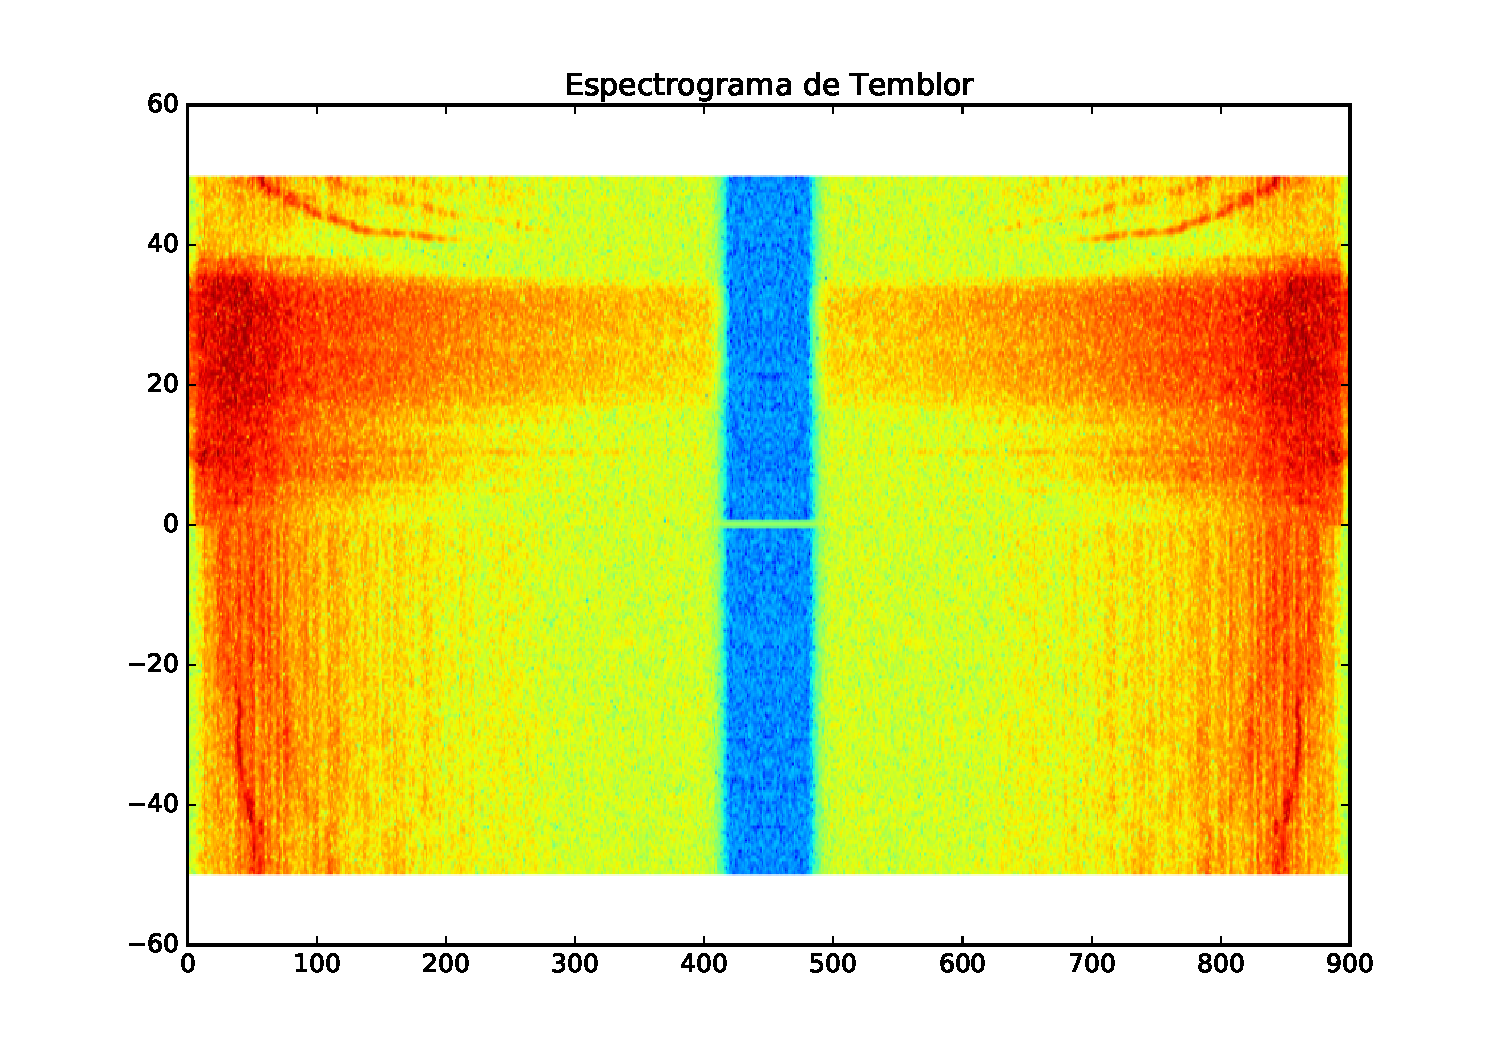
\includegraphics[width=14cm]{2_EspectrogramaTemblor.pdf}
\end{center}
Espectrograma del temblor. Acá se puede ver, de nuevo, la concentración de frecuencias alrededor de \textbf{ PEDIENTE }.

\section{Ejercicio 3: Ecuaciones diferenciales - edificio en un sismo}
\begin{center}
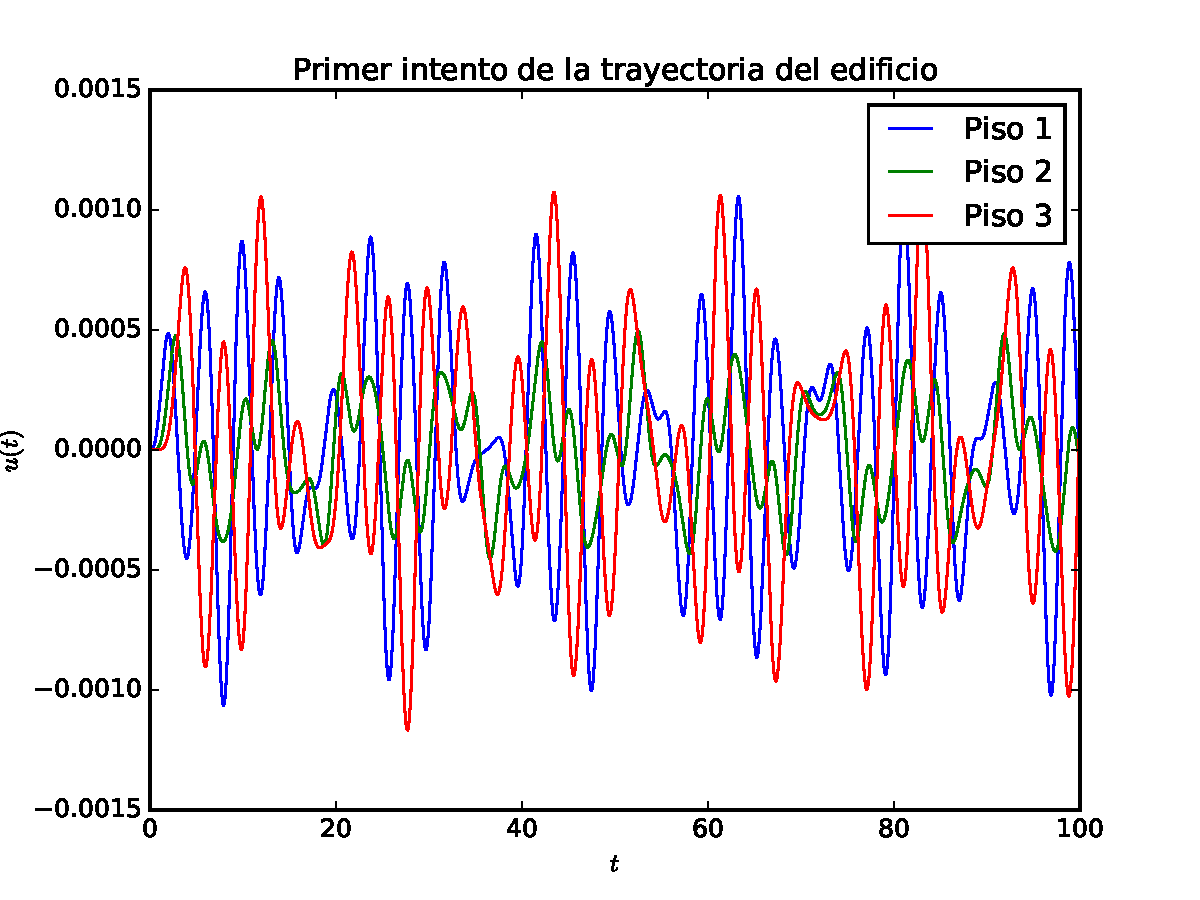
\includegraphics[width=14cm]{3_PrimerEdificio.pdf}
\end{center}
Gráfica de la trayectoria del centro de masa de cada piso $u_i(t)$ durante un sismo que ejerce una fuerza periódica $F(t)=\sin(\omega t)$ con $\omega=\sqrt{\frac{k}{m}}$ donde $k$ modela la rigidez de la estructura y $m$ la masa de cada piso. Para esta frecuencia en particular los pisos 1 y 3 oscilan con mayor amplitud que el segundo piso, que parece más estable.
\begin{center}
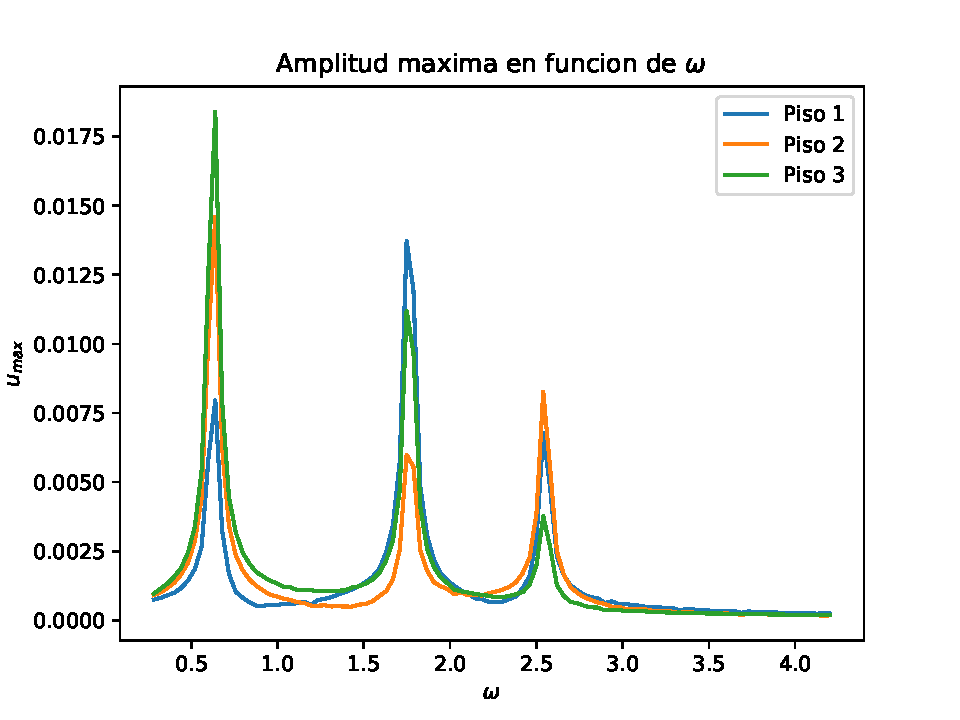
\includegraphics[width=14cm]{3_Maximos.pdf}
\end{center}
Gráfica de la amplitud máxima de la oscilación $u_{max}$ de cada piso en función de la frecuencia del sismo $\omega$ en el intervalo $\left[0.2\sqrt{\frac{k}{m}},3\sqrt{\frac{k}{m}} \right]$. Se pueden ver claramente tres picos, las cuales corresponderán a un tipo particular de resonancia del edificio. Usando Python podemos ver que 0.639225,1.74797,2.53993

\end{document}
